\subsection{Design du filtre numérique}
Pour concevoir les différents étages du filtre numérique, le code Python mis à notre disposition dans le cadre du projet est \textit{digitalFilterDesign.py}. Les filtres passe-bande ont été conçus selon les spécifications suivantes pour chaque fréquence centrale.

\subsubsection{Filtre Passe-Bande à 900 Hz}
\begin{itemize}
\item Fréquence d'échantillonnage : 16000 Hz
\item Fréquence centrale : 900 Hz
\item Largeur de la bande passante : 27 Hz
\item Gain minimum dans la bande passante : 0.9
\item Largeur de la bande bloquante : 63 Hz
\item Gain maximum dans la bande bloquante : 0.1
\end{itemize}

Les coefficients des étages du filtre sont les suivants :
\begin{align*}
    H_1(z) &= 0.001771 \frac{1+2z^{-1}+z^{-2}}{1-1.86370006z^{-1}+0.98824962z^{-2}} \\
    H_2(z) &= 0.001726 \frac{1+2z^{-1}+z^{-2}}{1-1.86719114z^{-1}+0.98840267z^{-2}} \\
    H_3(z) &= 0.023 \frac{1-2z^{-1}+z^{-2}}{1-1.86766577z^{-1}+0.99507105z^{-2}} \\
    H_4(z) &= 0.02283 \frac{1-2z^{-1}+z^{-2}}{1 -1.87591938z^{-1}+ 0.99522511z^{-2}}
\end{align*}
Le gain maximum des étages est 1.6757.

\begin{figure}[H]
    \centering
    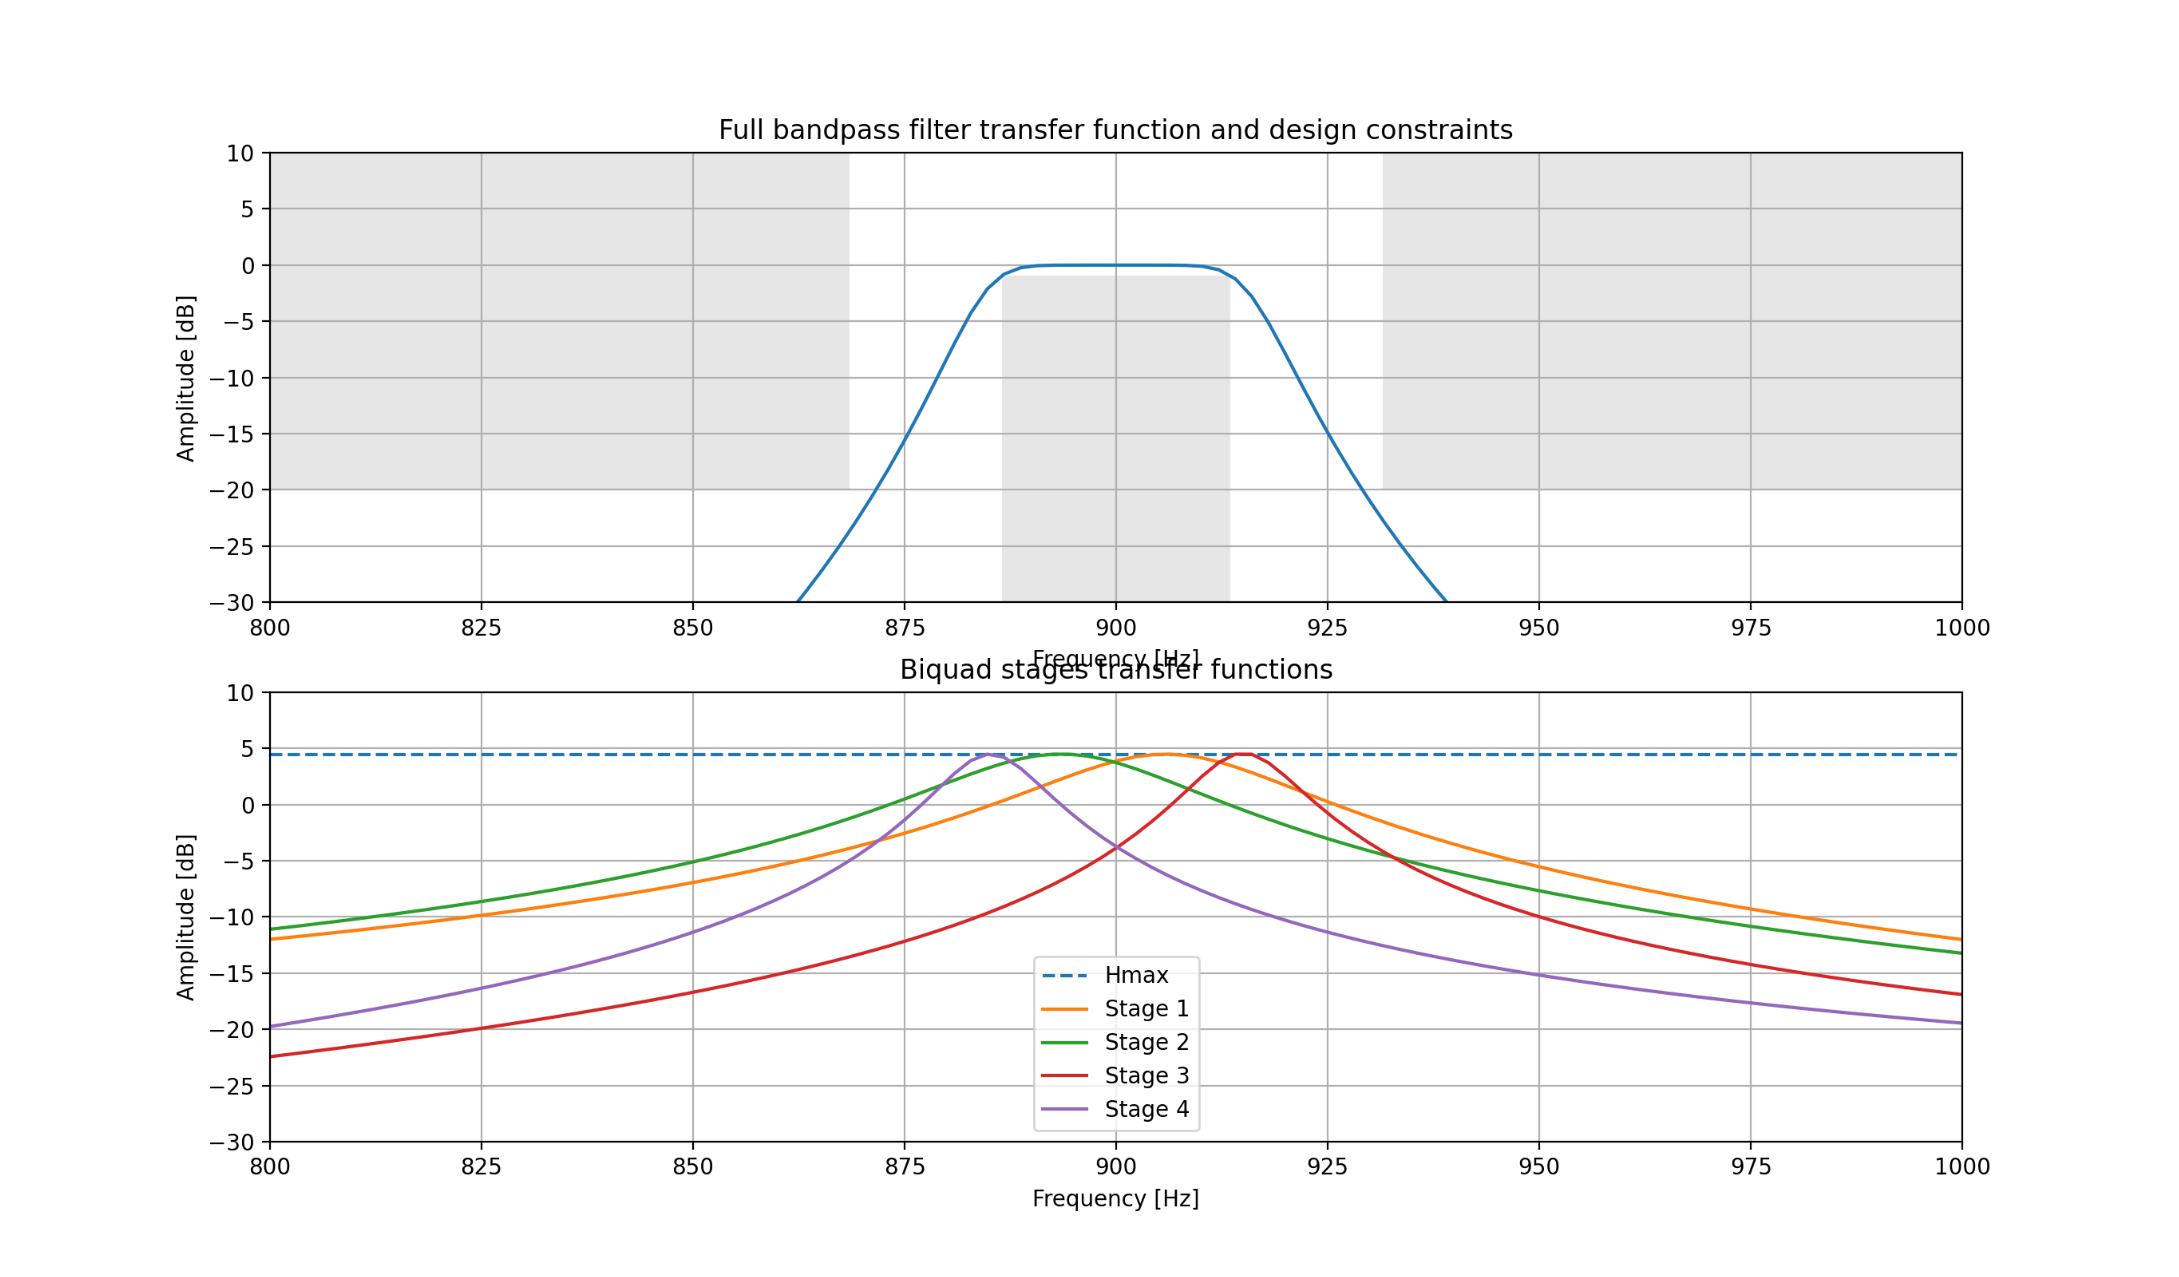
\includegraphics[width=0.7\textwidth]{Pictures/filtre iir 900.png}
    \caption{Filtre passe bande et des différents étages pour la fréquence centrale à 900Hz}
    \label{fig:enter-label}
\end{figure}

\subsubsection{Filtre Passe-Bande à 1100 Hz}
\begin{itemize}
    \item Fréquence d'échantillonnage: 16000 Hz
    \item Fréquence centrale: 1100 Hz
    \item Largeur de la bande passante: 33 Hz
    \item Gain minimum dans la bande passante: 0.9
    \item Largeur de la bande bloquante: 77 Hz
    \item Gain maximum dans la bande bloquante: 0.1
\end{itemize}

Les coefficients des étages du filtre sont les suivants:
\begin{align*}
    H_1(z) &= 0.00259 \frac{1+2z^{-1}+z^{-2}}{1-1.80592184z^{-1}+0.98584165z^{-2}} \\
    H_2(z) &= 0.002661 \frac{1+2z^{-1}+z^{-2}}{1-1.80081358z^{-1}+0.98565917z^{-2}} \\
    H_3(z) &= 0.02277 \frac{1-2z^{-1}+z^{-2}}{1-1.8047745z^{-1}+0.99398116z^{-2}} \\
    H_4(z) &= 0.02273 \frac{1-2z^{-1}+z^{-2}}{1-1.8169234z^{-1}+0.99416513z^{-2}}
\end{align*}
Le gain maximum des étages est 1.6796.
\begin{figure}[H]
    \centering
    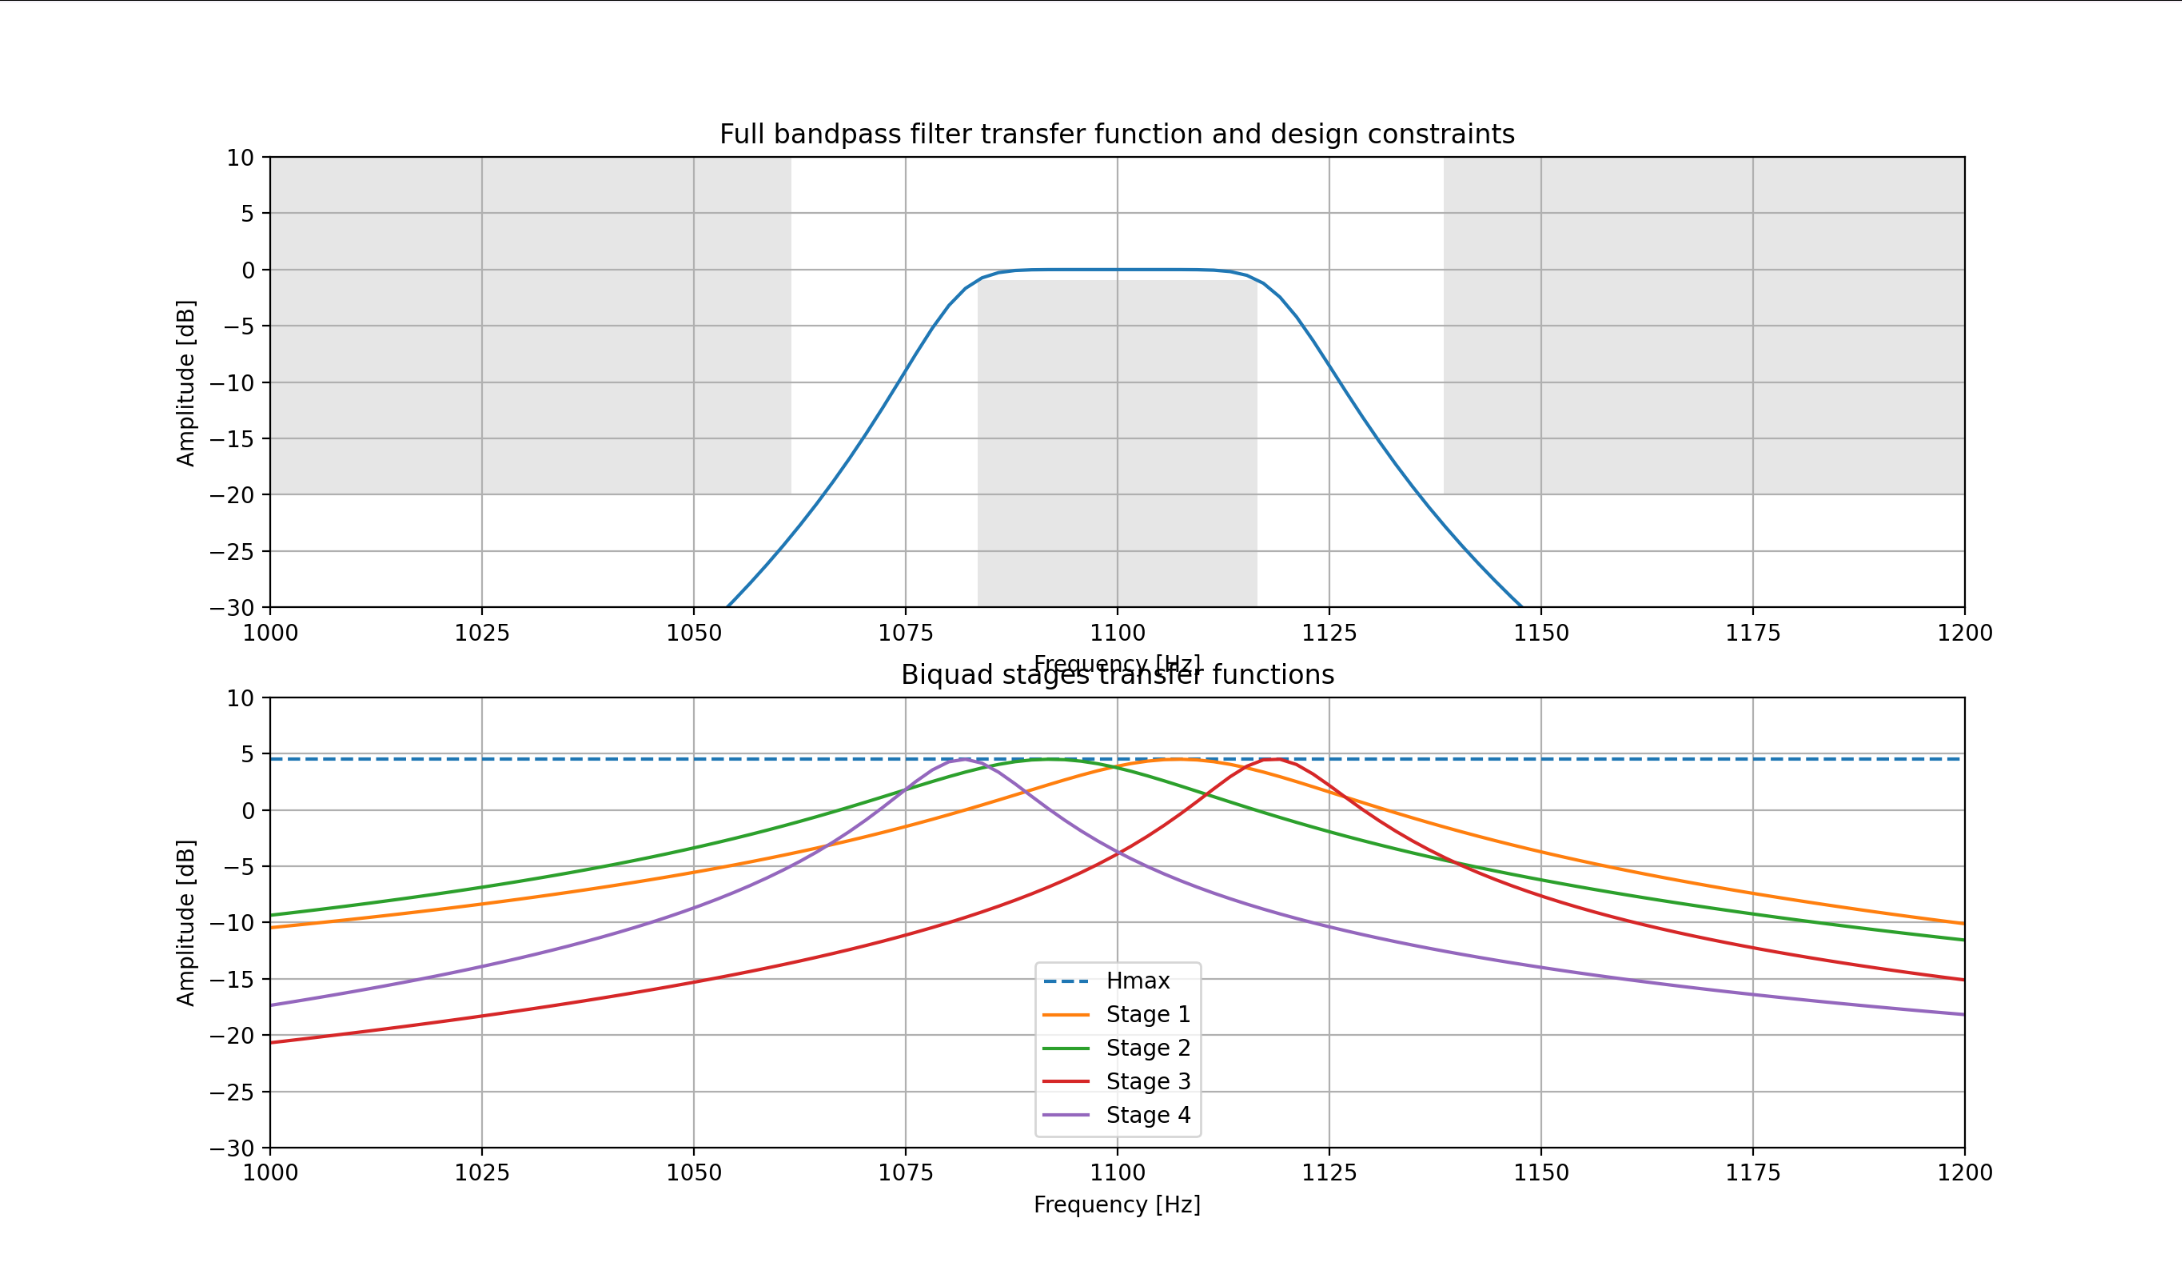
\includegraphics[width=0.7\textwidth]{Pictures/filtre iir 1100.png}
    \caption{Filtre passe bande et des différents étages pour la fréquence centrale à 1100Hz}
    \label{fig:enter-label}
\end{figure}


